\chapter{Datenassoziationen}\label{chapter:association}

Wie in der Einleitung beschrieben, soll in einem ersten Ansatz analysiert werden, ob eine TSDF Karte mit gegebenem initialen Pfad durch die Optimierung des initalen Pfades mittels Schleifenschlüssen verbessert werden kann. Die Grundlage für die Optimierung der Karte ist zu identifizieren, welcher Teil der Karte bei einer Veränderung der Trajektorie mit transformiert werden muss. Dies Kapitel befasst sich mit der Generation von Datenassoziationen zwischen den Posen des Pfades und der TSDF-Karte.

\section{Ansatz}
\label{section:ansatz}

Wie bereits in Kapitel \ref{section:tsdf} beschrieben, wird die TSDF Karte in \cite{HATSDF} inkrementell erweitert, sobald eine definierte minimale Distanz zurückgelegt wurde. Dabei werden nicht nur neue Zellen beschrieben, sondern auch die Werte bereits beschriebener Zellen gewichtet verändert. Dementsprechend kann die Information in einer Zelle eine Akkumulation beliebig vieler Updates sein, also beliebig vielen Posen zugeordnet werden. Diese Information gilt es zu berücksichtigen, wenn auf Basis einer gegebenen TSDF Karte Datenassoziationen identifiziert werden sollen.
Eine Möglichkeit der Generation dieser Assoziation wäre eine \textbf{1:1} Beziehung zwischen den Zellen und Posen aufzubauen. Dann würde eine Zelle maximal einer Pose zugeordnet werden. Da bereits bekannt ist, dass eine Zelle von mehreren Posen angepasst werden kann, ist diese Art der Beziehung zwischen Posen und TSDF-Zellen allerdings von einem großen Informationsverlust geprägt. Die Alternative zur \textbf{1:1} Beziehung ist eine \textbf{1:N} Beziehung zwischen einer Zelle und $N$ Posen. Diese Beziehung ist aufgrund der genannten Eigenschaften des TSDF-Karten Updates der \textbf{1:1} Beziehung zu bevorzugen.

Die Informationen darüber, welche Position welche TSDF Zelle beschrieben lässt sich allerdings nicht ohne Weiteres aus der TSDF Karte herauslesen.
Um dies zu ermöglichen könnte \cite{HATSDF} um die Funktion erweitert werden an jeder Zelle zusätzlich ein Array zu speichern, in dem die Posen enthalten sind, die die betroffene Zelle modifiziert haben. Dieses Array muss in einem eigenen Datenset gespeichert sein, da die Anzahl Posen, die auf diese Weise einer Zelle zugeordnet werden können, dynamisch ist. Das bedeutet, dass für jede einzelne TSDF Zelle ein eigenes Datenset gespeichert werden muss, in dem die zugehörigen Posen enthalten sind. Je nach Auflösung der diskretisierten Karte müssten nach diesem Ansatz mehrere Millionen separate Datensets gespeichert werden. Ein solches Vorgehen erfordert nicht nur viel Speicher, sondern ist auch aus hierarchischer Betrachtungsweise keine sinnvolle Herangehensweise.
\improvement{TODO: anhand mehrerer Datensätze Assozationen bilden und schauen, von wie vielen Posen eine Zelle im Durchschnitt angepasst wurde und hochrechnen, was das für den Speicher bedeutet}
%Eine andere Möglichkeit wäre \cite{HATSDF} so zu erweitern, dass für jede Pose $P_t$ die Koordinaten der TSDF Zellen gespeichert werden, die im Zeitschritt beziehunsweise Inkrement $t$ angepasst wurden.
Eine Möglichkeit, die gewünschten Daten auf Basis einer gegebenen TSDF Karte zu generieren ist diese über die Methode, mit der die Daten generiert wurden, zu regenerieren. In \cite{HATSDF} wird die TSDF-Karte über ein \textbf{Ray-Marching} generiert. Eine alternative zum Ray-Marching stellt der Bresenham Algorithmus dar, der die Diskretisierung der Karte ausnutzt.
Beide Varianten werden im Folgenden beschrieben, evaluiert und miteinander verglichen.

Zunächst beschreibt die folgende Sektion die Speicherung der Datenassoziation in der HDF5-Datenstruktur.

\section{Serialisierung}

Diese Sektion beschreibt, wie identifizierte Assoziationen in der HDF5-Datei gespeichert werden, die Daten der Karte enthält.
Wie bereits zuvor beschrieben, enthält die HDF5 Struktur mehrere Gruppen, die jeweils weitere Daten enthalten. Zu diesen Gruppen gehören in diesem Fall \textit{/map} und \textit{/poses}.
Die Map-Gruppe enthält dabei die serialisierten TSDF-Zellenwerte und TSDF-Zellengewichte. Die Poses-Gruppe enthält die serialisierten 6D Posen des Pfades als Datensets.
Der HDF5 interne Pfad eines dieser Pose-Datensets ist \textit{/poses/[index]}, wobei \textit{index}, der Index der Pose im Pfad ist.
An dieser Stelle wird nun einer Erweiterung vorgenommen um die generierten Assoziationen zu serialisieren. Anstelle der Datensets wird für jede Pose eine eigene Gruppe erstellt. Diese Gruppe erhält als Namen ebenfalls den Pfadindex der Pose. Innerhalb dieser Gruppe wird ein Datenset für die Pose und optional ein weiteres Datenset für die Datenassoziationen angelegt, sofern erforderlich.
Abbildung \ref{fig:hdf5new} zeigt die neue interne HDF5 Struktur nach dieser Änderung.

\begin{figure}
		\centering
		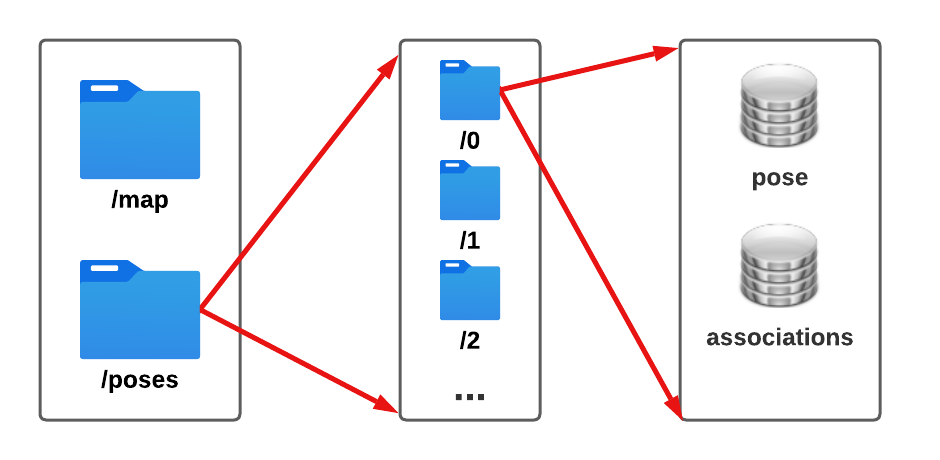
\includegraphics
			[scale=0.4]
			{HDF5new}
		\caption
			[Caption for LOF]{Schematische Darstellung der HDF5 internen Datenstruktur nach Speicherung der generierten Datenassoziationen zwischen TSDF-Zellen und Posen. Die in Kapitel \ref{section:ansatz} beschrieben \textit{1:N} Beziehung zwischen einer Zelle und den zugehörigen Posen ist hier indirekt realisiert. Anstelle pro Zelle ein Datenset zu erstellen, wir für jede Pose ein Datenset enthält, das alle assoziierten TSDF-Zellen enthält. Verschiedene Posen können dabei dieselbe TSDF-Zelle assoziieren. Das Datenset \textit{pose} enthält die Transformation der aktuellen Pose ins Urpsrungskoordinatensystem. Das Datenset \textit{associations} enthält ein Array der assoziierten Zellkoordinaten, die durch die Diskretisierung ganzzahlig sind und als Integer abgespeichert werden.}			                                                                                                                                     
		\label{fig:hdf5new}
\end{figure}

Auf Basis dieser Änderungen wird im Folgenden erläutert, wie die zu speichernden Zellen für jede Pose ermittelt werden.

\section{Algorithmen}

Diese Sektion stellt die Algorithmen heraus, mit denen beschriebene Assoziationen identifiziert werden können. Die Ergebnisse der Algorithmen werden miteiander verglichen und evaluiert.

\subsection{Ray-Tracing}

Eine Möglichkeit der Ermittlung der mit einzelnen Posen assoziierten Teilbereiche der TSDF Karte ist die die Erstellung eines künstlichen Laserscans innerhalb der TSDF Karte, ausgehend von der entsprechenden Pose.
Entsprechend wurde im Zuge dieser Arbeit ein \textbf{Ray-Tracer} entwickelt, der künstliche Laserstrahlen innerhalb der TSDF-Karte aussendet und die Schnittpunkte mit der TSDF Karte überprüft. Der Ray-Tracer ist beliebig konfigurierbar ist und kann an die Parameter verschiedenster Laserscanner angepasst werden.
Die wesentlichen Parameter und deren Bedeutung sind Tabelle \ref{table:raytracer_params} zu entnehmen.
	
	\begin{table}
		\centering
		\caption{Parameter des in dieser Arbeit entwickelten Ray-Tracers zur Bestimmung des mit einer beliebigen Pose assoziierten Teilbereichs der TSDF-Karte. Der horizontale Öffnungswinkel wird an dieser Stelle als $360$ Grad angenommen.}
		\begin{tabular}{| p{3cm} | p{8cm} | p{2cm} |}
			\hline
			\thead{Parameter}   & \thead{Funktionsweise}  & \thead{Default-\\Wert}\\
			\hline
			$opening\_degree$   & Definiert den vertikalen Öffnungswinkel des Ray-Tracers. Anzugeben in Grad. & $45$ \\
			\hline
			$hor\_res$     & Definiert die horizontale Auflösung des Laserscanners. Der gegebene Wert  entspricht der Anzahl \textit{Rays} pro Scanebene. & $1024$\\
			\hline			
			$vert\_res$    & Definiert die vertikale Auflösung des Laserscanners. Der gegebene Wert entspricht der Anzahl an Scanebenen im Laserscan. & $128$\\
			\hline			
			$step\_size$      & Definiert, wie groß die Schrittweite beim Aussenden der einzelnen Rays ist. Der Wert ist in Metern anzugeben. Der Default-Wert ist direkt an die Zellgröße der diskreten TSDF-Karte $map_{res}$ gekoppelt und beträgt $\frac{map_{res}}{2}$. & $0.032$ \\
			\hline			
			$ray\_size$   & Definiert die Dicke des Strahls in der Visualisierung. Dieser Parameter dient lediglich zur erleichterten Visualisierung des Laserscans bei unterschiedlicher Konfiguration. Der Wert ist in Metern anzugeben. & $0.01$ \\
			\hline
		\end{tabular}
		\label{table:raytracer_params}
	\end{table}	
	
Zur Emulation das Laserscans wird zunächst ein Array erstellt, in dem die aktuellen Endpunkte der jeweiligen Rays gespeichert werden. Die Anzahl an Endpunkten $n$ ist definiert durch die konfigurierte Auflösung. Sie beträgt:

\begin{myequation}
n = vert\_res \cdot hor\_res
\end{myequation}

 Der Startpunkt jedes Rays ist die Pose $P_i$, von der aus der Laserscan ausgesendet wird. Ziel ist in jeder Iteration alle Rays um $step\_size$ zu verlängern und die TSDF-Zellen zu evaluieren, die derzeit von den einzelnen Rays getroffen werden. Für diese Verlängerung der Rays müssen diese zunächst initialisiert werden. Diese Initialisierung erfolgt auf Basis der parametrisierten Öffnungswinkel des Laserscanners $opening\_degree\_vert$ und $opening\_degree\_hor$, sowie der konfigurierten vertikalen und horizontalen Auflösung $vert\_res$ und $hor\_res$.
Zunächst werden die Winkelbereiche definiert, in den der Ray-Tracer operiert. Diese setzten sich aus den Öffnungswinkeln zusammen. Der Winkelbereich in horizontaler Richtung beträgt:

\begin{myequation}
I_{hor} = \left[-opening\_degree\_hor, opening\_degree\_hor \right]
\end{myequation}

Der Winkelbereich in vertikaler Richtung beträgt:

\begin{myequation}
I_{vert} = \left[-opening\_degree\_vert, opening\_degree\_vert \right]
\end{myequation}

Die jeweiligen Winkelbereiche werden durch die konfigurierte Auflösung diskretisiert.
Die horizontale Schrittweite des Laserscanners beträgt:

\begin{myequation}
\Delta_{hor} = \frac{opening\_degree\_hor}{hor\_res}
\end{myequation}

Die vertikale Schrittweite des Laserscanners beträgt:

\begin{myequation}
\Delta_{vert} = \frac{opening\_degree\_vert}{vert\_res}
\end{myequation}

Basierend auf den unteren und oberen Winkelschranken und der berechneten Schrittweite zwischen diesen Schranken kann nun das Array initialisiert werden. Dazu wird in zwei Schleifen über die beiden Winkelintervalle $I_{vert}$ und $I_{hor}$ iteriert und der aktuelle Wert jeweils um die berechneten Delta $\Delta_{vert}$ und  $\Delta_{hor}$ inkrementiert. Aus den beiden Winkeln $\alpha$ und $\beta$ der aktuellen Iteration der Schleifen, sowie einer beliebigen Distanz initialen Länge des Rays, wie zum Beispiel der Schrittweite $step\_size$ können nun für jeden Punkt die initialen Ray-Punkte berechnet werden, die den Richtungsvektor des Rays definieren.
Hierzu ist eine Umwandlung von Kugelkoordinaten in das Kartesische Koordinatensystem notwendig. Mit $alpha$, $beta$ und $step\_size$ wird in Kugelkoordinaten genau ein Punkt im dreidimensionalen Raum beschrieben. Um diese in kartesische Koordinaten im ROS Koordinatensystem umzuwandeln wird folgende Formel verwendet ($\alpha$ und $\beta$ gegeben in Radianten, $\alpha$ beschreibt den aktuellen Winkel um die z-Achse, $\beta$ die aktuelle Rotation um die y-Achse):

\begin{myequation}
\colvec{x_{P_i}\\y_{P_i}\\z_{P_i}} = step\_size \cdot \colvec{\cos\left(\alpha \right) \cdot \cos\left(\beta \right) \\ \sin\left(\alpha \right) \cdot \cos\left(\beta \right) \\ \sin\left(\beta \right)}
\end{myequation}

Der Punkt $\colvec{x_{P_i}\\y_{P_i}\\z_{P_i}}$ beschreibt hier zunächst nur den Ray-Punkt aus Sicht des lokalen Map-Koordinatensystems, das durch ${P_i}$ beschrieben ist. Um diesen aus Sicht des globalen Koordinatensystems $\mathbb{M}$ zu betrachten, muss dieser Punkt dorthin transformiert werden. Grundlagen zur Transformation werden in Kapitel \ref{section:transformationen} behandelt. Es ist essentiell, dass an dieser Stelle nicht nur die Translation, sondern auch die Rotation berücksichtigt wird um den Scan von Pose $P_i$ bestmöglich replizieren zu können. Die Transformation des Vektors $\colvec{x_{P_i}\\y_{P_i}\\z_{P_i}}$ vom Koordinatensystem beschrieben durch Pose $P_I$ in das globale Koordinatensystem $\mathbb{M}$ mit der Transformationsmatrix $T_{P_i \rightarrow \mathbb{M}}$ ist gegeben durch:

\begin{myequation}
\colvec{x_{\mathbb{M}}\\y_{\mathbb{M}}\\z_{\mathbb{M}}} = T_{P_i \rightarrow \mathbb{M}} \cdot \colvec{x_{P_i}\\y_{P_i}\\z_{P_i}}
\end{myequation}

Auf diese Weise werden alle initialen Endpunkte des emulierten Laserscans berechnet. Auf Basis der berechenten initialen Endpunkte und des bekannten Anfangspunktes gegeben durch den Translationsanteil von $P_i$ kann das inkrementelle Ray-Tracing beginnen.
In jeder Iteration des Ray-Tracing werden alle Rays um $step\_size$ verlängert und die entsprechend getroffenen Zellen evaluiert. Um einen Vektor $\vec{v}$ gegeben durch den Translationsanteil $\vec{t_i}$ und den aktuellen Endpunkt des betrachteten Rays $\vec{r_i}$ um $step\_size$ zu verlängern und daraus den neuen Endpunkt des Rays $\hat{\vec{r_{i}}}$ zu berechnen wird folgende Formel verwendet:

\begin{myequation}
\hat{\vec{r_{i}}} = \frac{\norm{\vec{r_i} - \vec{t_i}} + step\_size}{\norm{\vec{r_i} - \vec{t_i}}} \cdot \left( \vec{r_i} - \vec{t_i} \right) + \vec{t_i} 
\end{myequation}

Nach der Verlängerung eines Rays $\vec{r_i}$ wird die inder aktuellen Iteration $j$ getroffene TSDF-Zelle $C_i^j$ evaluiert. Je nach Schrittweite $step\_size$ und Auflösung des Ray-Tracers ist es möglich, dass $C_i^j$ bereits evaluiert wurde und schon eine Assoziation mit der Pose $P_i$ hergestellt ist. Um diesen Fall zu überprüfen und zu verhindern, dass duplizierte Assoziationen gespeichert werden, wird eine Hash-Map genutzt, deren Hash auf Basis der Koordinaten der TSDF-Zelle berechnet wird. Ist $C_i^j$ bereits in der Hash-Map gespeichert, ist der aktuell betrachtete Ray $\vec{r_i}$ für diese Iteration fertig evaluiert und der nächste Ray kann betrachtet werden. Um zu entscheiden ob eine nicht assoziierte Zelle $C_i^j$ als Assoziation in Frage kommt müssen mehrere Zustände des Rays definiert werden. Abbildung \ref{fig:RayTracingBig} zeigt die benötigten Zustände und die Bedinungen für einen Wechsel des Status gegeben den aktuellen Status und die betrachtete Zelle $C_i^j$, sowie dieren TSDF-Wert und TSDF-Gewicht. Ein Ray ist beschränkt durch die lokale Karte um $P_i$ \ref{section:tsdf_map}, sowie die Struktur der TSDF-Karte. Detektiert ein Ray einen einen Wechsel von positive auf negative TSDF-Werte (\textbf{Nulldurchgang}) in der TSDF, stoppt der Ray-Tracer, sobald er erneut positive Werte detektiert. Diese Herangehensweise sorgt dafür, dass mit der Pose $P_i$ keine Zellen assoziiert werden, die von dieser Pose aufgrund der Begrenzungen der lokalen Karte nicht gesehen werden konnten oder hinter Wänden befindlich sind.

\begin{figure}
		\centering
		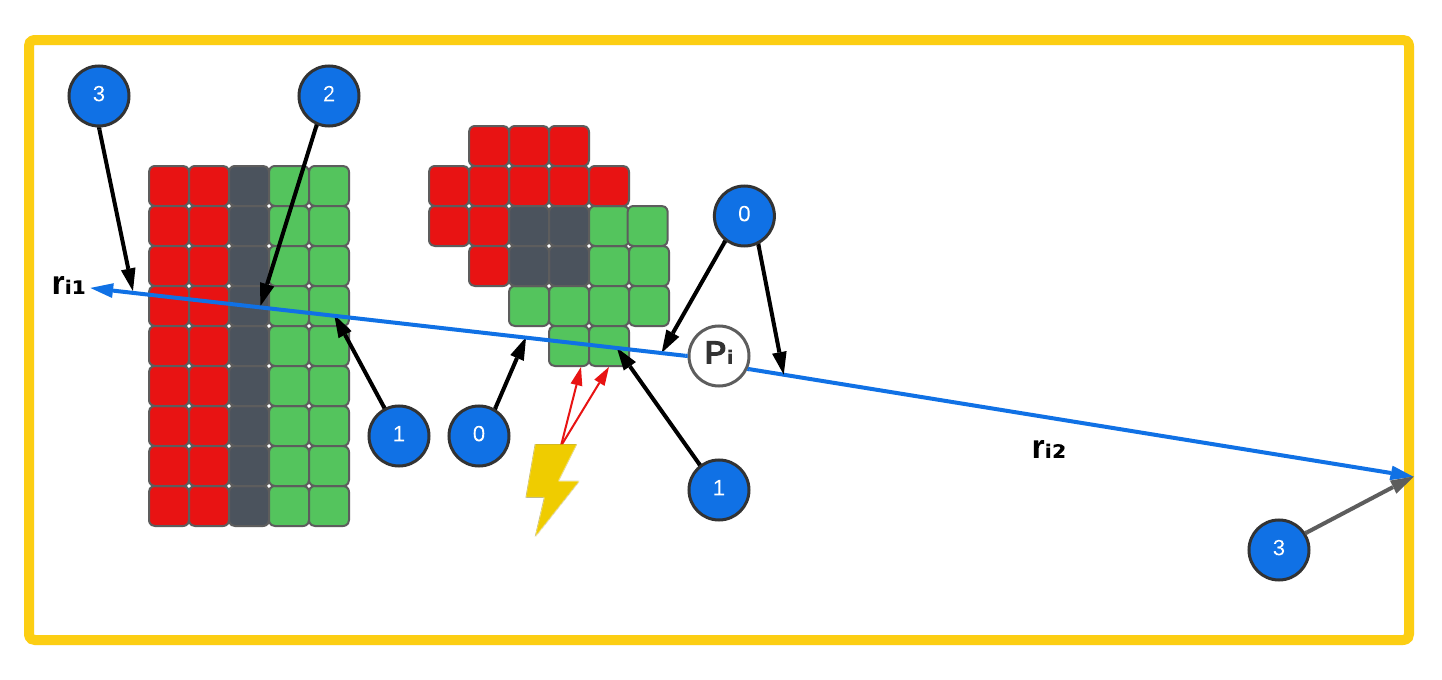
\includegraphics
			[scale=0.3]
			{RayTracingBig}
		\caption
			[Caption for LOF]{Schematische Darstellung 2D Darstellung der verschiedenen Zustände eines einzelnen Rays des Ray-Tracers innerhalb einer TSDF-Darstellung. Negative TSDF-Werte dargestellt in rot, positive in grün. Der approximierte Nulldurchgang in der TSDF ist hier gräulich dargestellt, die umgebende lokale Karte in gelb. Ausgehend von Pose $P_i$ sind zwei Rays $r_{i1}$ und $r_{i2}$ dargestellt, die die verschiedenen Fälle abdecken, die es zu berücksichtigen gilt. Eine genaue Beschreibung der Zustandsänderungen der Rays im Zustandsdisgramm \ref{fig:Ray-Trace-Zustandsdiagramm} zu entnehmen. Die entsprechenden Zustände sind dargestellt als blaue Kreise, die die jeweilige Zustandsnummer enthalten. Die entsprechenden Definitionen der Zustände sind ebenfalls im Zustandsdiagramm \ref{fig:Ray-Trace-Zustandsdiagramm} zu entnehmen. Die mit einem Blitz markierten Zellen werden zwar von dem ausgesandten Ray $r_{i1}$ getroffen, dürfen allerdings aufgrund der Evidenz im aktuellen Ray nicht mit der Pose assoziiert werden, da im Anschluss an diese Zellen kein Nulldurchgang, sondern Freiraum folgt. Der Freiraum ist hier in weiß dargestellt und setzt sich aus den TSDF-Zellen zusammen, die Default-Werte enthalten und entsprechend außer der minimalen Entfernung $tau \left(\tau\right)$ zur Oberfläche, keine räumlichen Informationen besitzen. Gleicher Ausnahmefall tritt ein, wenn der Ray lediglich negative TSDF-Zellen trifft. Diese werden ebenfalls nicht aufgrund der Evidenz des betrachteten Rays mit der Pose assoziiert.}		                                                                                                                                     
		\label{fig:RayTracingBig}
\end{figure}

\begin{figure}
		\centering
		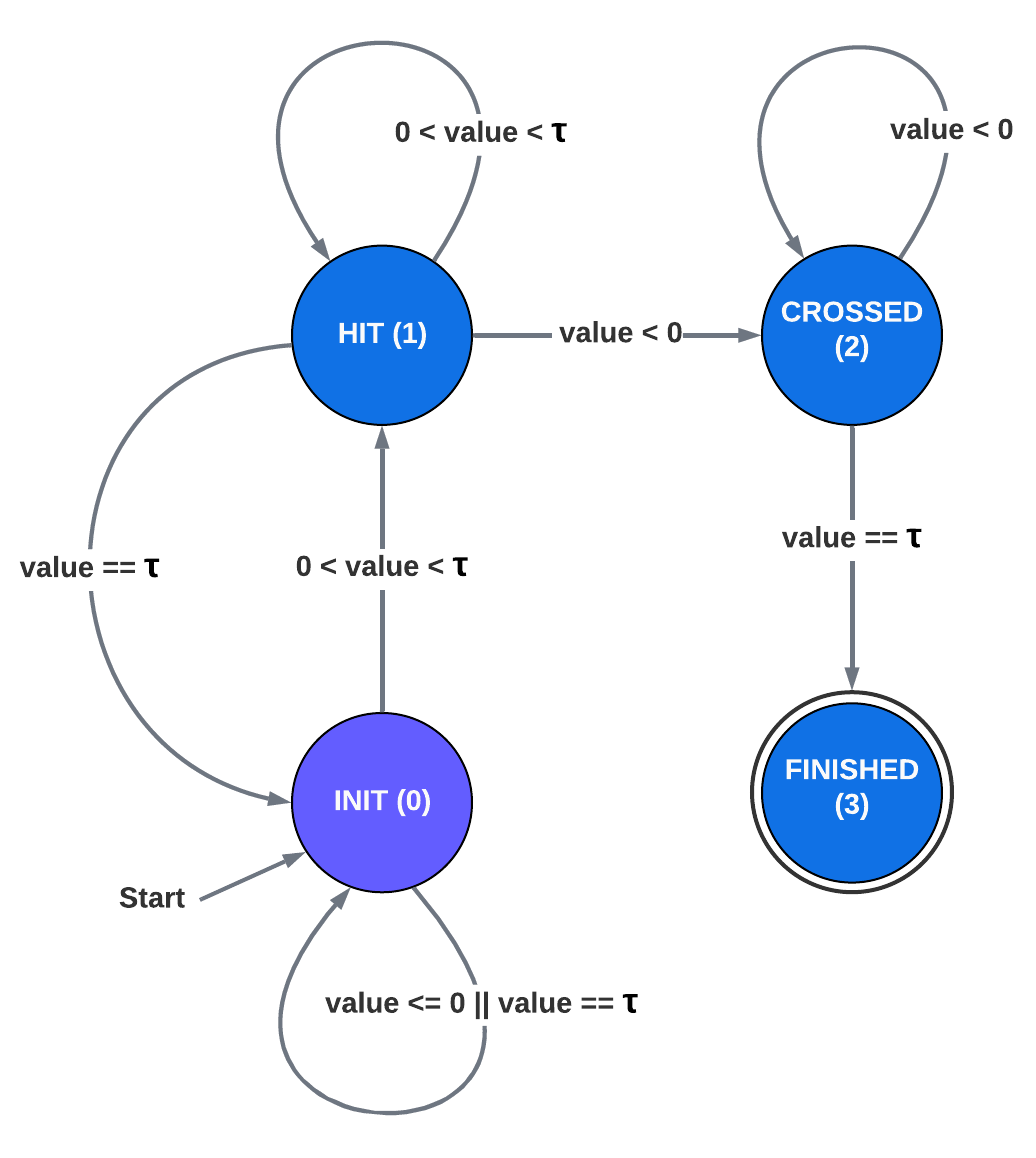
\includegraphics
			[scale=0.25]
			{Ray-Trace-Zustandsdiagramm}
		\caption
			[Caption for LOF]{Zustandsdiagramm der internen Zustände eines Rays. Zustandsübergänge sind beschrieben durch einen initialen Zustand und den TSDF-Wert der aktuellen Zelle (\textit{value}). In Zustand 1 werden gefundene Assoziationen zunächst nicht abgespeichert, da noch nicht bekannt ist, ob diese Zellen zu einem Nulldurchgang gehören oder ob der Ray nur Zellen kreuzt, die von einer anderen Pose aus befüllt wurden. Je nach TSDF-Wert der aktuellen Zelle werden die zwischengespeicherten Assoziationen aus Zustand 1 entweder verworfen oder in der HDF5 gespeichert.}		                                                                                                                                     
		\label{fig:Ray-Trace-Zustandsdiagramm}
\end{figure}

Die Ergebnisse dieses Ansatz sind in Abbildung \ref{fig:bresenham_vs_raytrace}im Vergleich mit den Ergebnisses des Bresenham Algorithmus dargestellt, der in der nachfolgenden Sektion behandelt wird. In dem genutzten Datensatz können nur etwa $91\%$ der Zellen assoziiert werden. Diese Zahl ähnelt auch der von Bresenham. \improvement{Für mehrere Datensätze zahlen bilden, graphlich darstellen}. Sektion \ref{section:association_evaluation} evaluiert die Ergebnisse von Ray-Tracing und Bresenham und vergleicht diese miteinander. Zudem wird Bezug zum Informationsverlust bei der Assoziationsidentifikation genommen.


\improvement{Beschreibung von Türen, Beschreibung von Problem wie Verdeckung durch Diskretisierung, ggf. Ray-Trace Bild, Beschreibung von Fallstricken: Nicht getroffene Zellen, Information loss}

\improvement{ggf. RVIZ-Bild des Ray-Tracing Markers}

\subsection{Bresenham}

Eine alternative algorithmische Herangehensweise an das beschriebene Problem der Assoziationsidentifikation ist die Nutzung des Bresenham-Algorithmus nach Bresenham \cite{bresenham1965algorithm}. Dieser wurde usprünglich verwendet, um einen digitalen Plotter mittels eines Computers zu kontrollieren und beliebige zweidimensionale Linien und Kurven approximativ abzubilden. Der Plotter lässt sich dabei in acht Richtungen auf einem diskretisierten Raster bewegen. Bresenham \cite{bresenham1965algorithm} beschreibt, wie sich die Zelle im Raster berechnen lässt, die das gegebene Liniensegment einer Kurve oder eine Linie selbst am besten beschreibt. Der Bresenham Algorithmus findet heutzutage vielfach Anwendung im Bereich der Computergrafik und wird verwendet. Hier liegt eine Diskretisierung durch die Auflösung des Computers in Pixeln vor. Mittels des Bresenham Algorithmus kann bestimmt werden, durch welche Pixel eine Linie oder ein Liniensegment beschrieben werden kann. Die in dieser Arbeit genutzte TSDF-Karte weist ebenfalls eine Diskretisierung auf, allerdings in drei Dimensionen.  

\improvement{Alles weiter unten ignorieren}


alternative Möglichkeit zur Identifikation von Assoziationen
gut nutzbar, da eine diskrete Karte vorliegt
Beschleunigung gegenüber RayTracing in reiner Software Variante erklären
Algorithmus erklären
Varianten der Bestimmung von start/endzelle bestimmen: Schnittpunkt zwischen Ray und lokaler Karte, über vektor und abfrage

\subsection{Ergebnisse}
\label{section:association_results}

\begin{figure}
	\centering
	\begin{subfigure}{.5\textwidth}
 		 \centering
  		 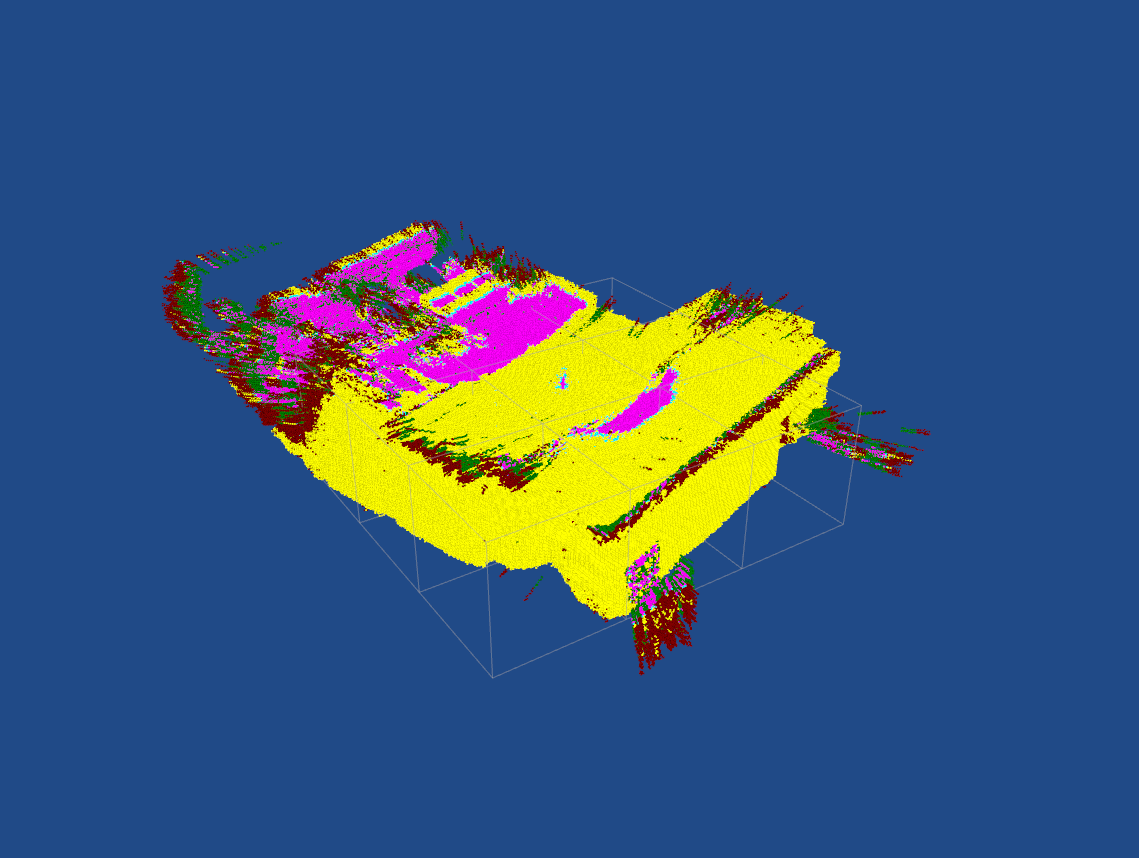
\includegraphics[width=.95\linewidth]{sp_bresenham_91_74_}
  		 \centering \caption{Assoziationen identifiziert mit Bresenham.}
  		 \label{fig:sp_bresenham}
	\end{subfigure}%
	\begin{subfigure}{.5\textwidth}
    	\centering
  		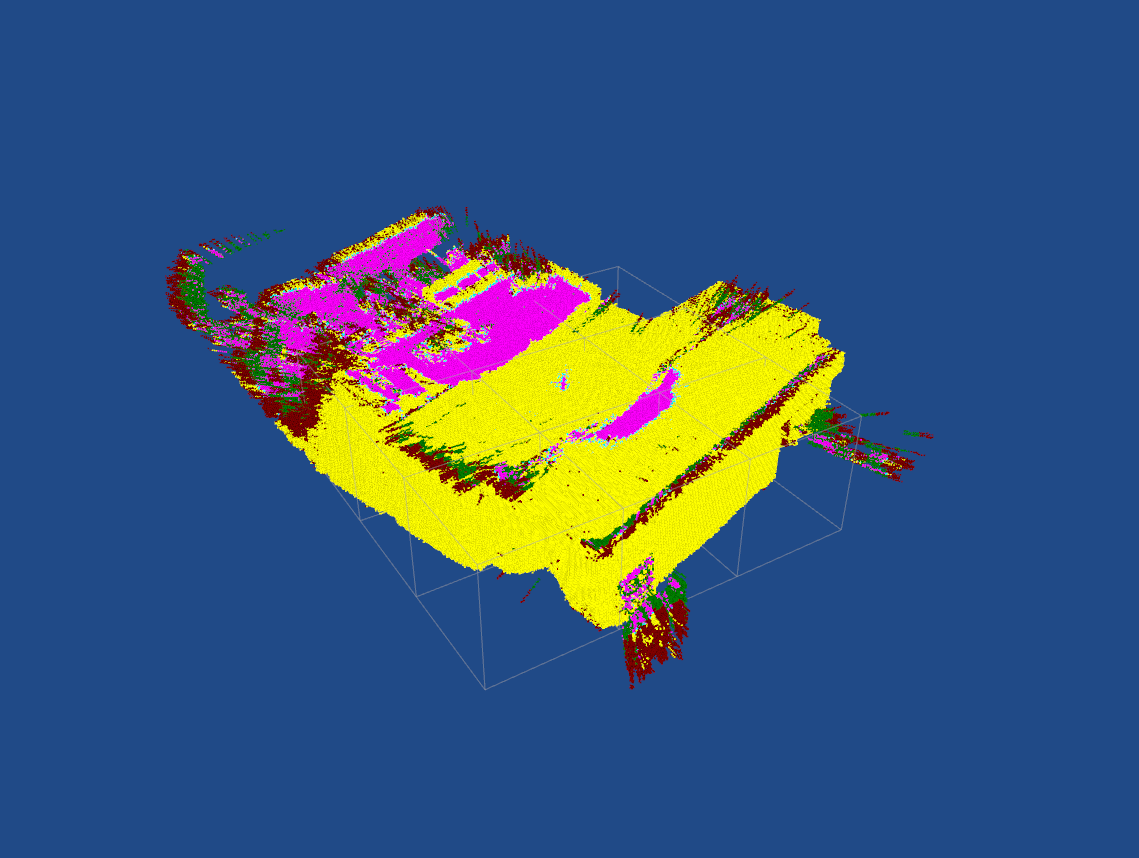
\includegraphics[width=.95\linewidth]{sp_raytrace_91_97_}
  		\centering \caption{Assoziationen identifiziert mit Ray-Tracing.}
  		\label{fig:sp_raytrace}
	\end{subfigure}
	\caption{Gegenüberstellung der generierten Assoziationen für einen Beispieldatensatz. Die durch Bresenham gefunden Assoziationen sind auf der linken Seite, die durch Ray-Tracing auf der rechten dargestellt. In diesem Fall wurden von Bresenham $91,74$ Prozent der Zellen assoziiert, während vom Ray-Tracing $91,97$ Prozent der Zellen assoziiert wurden. Zellen in gelb: assoziierte TSDF Zellen mit $value < 0$, Zellen in pink: assoziierte TSDF Zellen mit $value > 0$, Zellen in türkis: approximierter Nulldurchgang (Wechsel von positivem zu negativem Wert), Rest: nicht assoziierte Zellen. Zellen die nicht assoziiert werden, sind in diesem Fall größtenteils Teil von Verdeckungen oder Reflektionen des Laserscans und können als Outlier identifiziert werden.}
	\label{fig:bresenham_vs_raytrace}
\end{figure}

\subsection{Evaluation}
\label{section:association_evaluation}


\section{Loop Closure}

Problem Loop Closure als Post-Processing Schritt ohne passende Punktwolke erklären:
einzige Repräsentation der Umgebung ist Karte
scan-matching erfordert Punktdaten, Möglichkeit: Approximation von punktwolken, funktioniert auch sehr gut (Beispielbild), aber: Punktwolken einer falsch generierten Karte aufeinander matchen ergibt nicht besonders viel sinn.

\section{Kartenupdate}

Beschreibung des Updates des ersten Ansatzes:
Beschreibung der drei Stufen und wie diese ermittelt wurden.
Beschreibung Hindernisse und Lösungen (Hashmaps)
Bezug zu Performanz der Hashmaps für diesen Fall (string, int, Vector3i)
-> kleines Benchmark

Beschreibung von Problemen:
Anschaulich erklären, wo es zu Problemen kommen kann (wenn benachbarte Zellen von unterschiedlichen Anzahl Posen "gesehen" wurden)

\subsection{Transformationen}



\improvement{Graph mit Prozenten Bresenham vs. Ray-Tracing bezüglich assoziierter Zellen, ggf. auch mit chemitz datenset}

Zum Test der ermittelten wurden auf den gegeben Pfad diverse Transformationen, wie das Verwischen \textbf{(Blur)} des Pfades, die Transformation oder Rotation des Pfades beziehungsweise eine Kombination mehrere Transformationen angewandt und auf Basis der Posedifferenzen ein Kartenupdate durchgeführt. Dies führte ebenfalls zu mehreren Problemen, insbesondere bei Rotationen.
Bilder für Translation, Blur, Rotation, Information loss (nicht getroffene Zellen) herausstellen, definieren wie dieser Information loss zustande kommt

\section{Evaluation}

Auf basis der vorigen sektionen erläutern, welche probleme es gibt, welche möglichen lösungsansätze es gibt und erklären, warum diese nicht weiter verfolgt wurden,
Überleitung in nächstes Kapitel (Loop Closures)
-> überlegen ob als nächstes kapiteö gegebenfalls das Kapitel über das map-update folgen sollte, damit die Überleitung sinnvoller ist



